% Created by tikzDevice version 0.12.6 on 2026-01-16 14:33:51
% !TEX encoding = UTF-8 Unicode
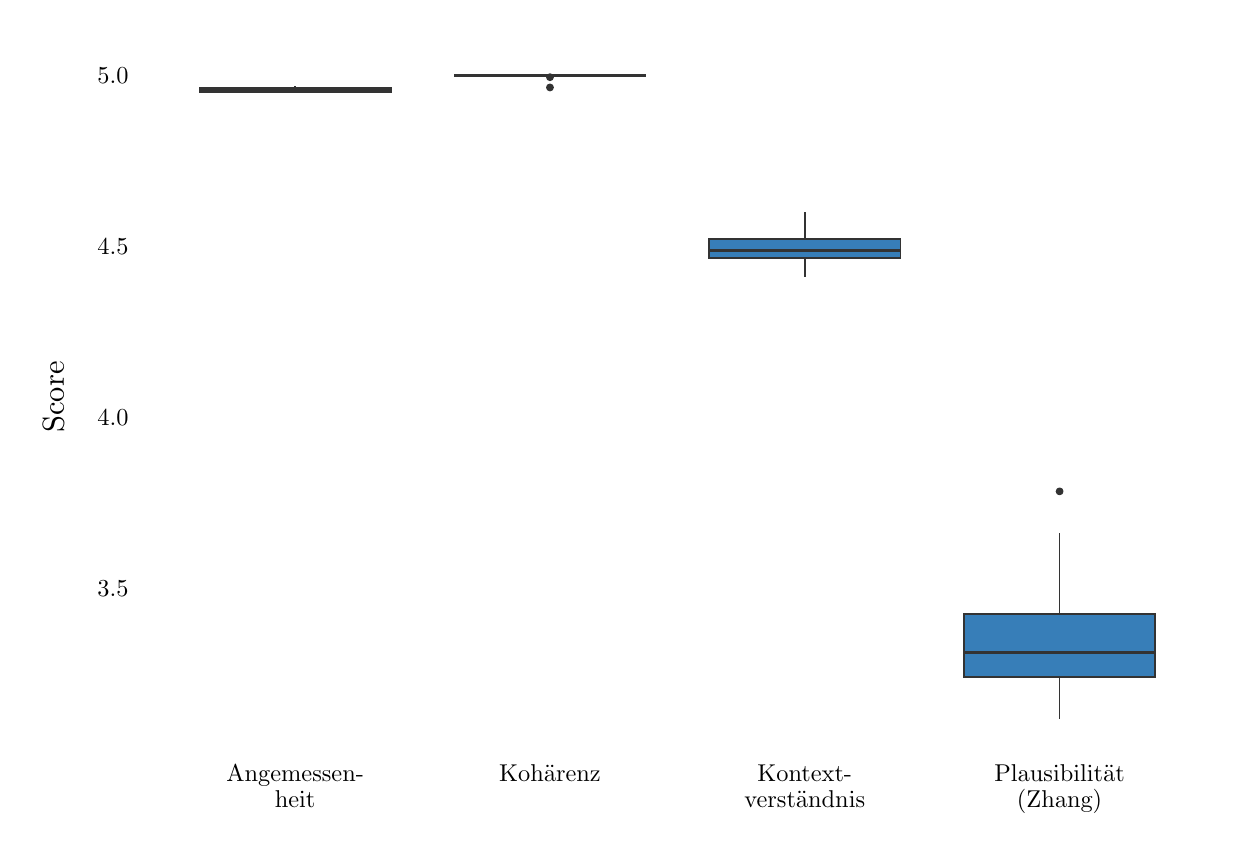
\begin{tikzpicture}[x=1pt,y=1pt]
\definecolor{fillColor}{RGB}{255,255,255}
\path[use as bounding box,fill=fillColor,fill opacity=0.00] (0,0) rectangle (433.62,289.08);
\begin{scope}
\path[clip] (  0.00,  0.00) rectangle (433.62,289.08);
\definecolor{fillColor}{RGB}{255,255,255}

\path[fill=fillColor] (  0.00,  0.00) rectangle (433.62,289.08);
\end{scope}
\begin{scope}
\path[clip] ( 41.41, 27.73) rectangle (428.12,283.58);
\definecolor{drawColor}{gray}{0.20}

\path[draw=drawColor,line width= 0.6pt,line join=round] ( 96.65,267.20) -- ( 96.65,267.93);

\path[draw=drawColor,line width= 0.6pt,line join=round] ( 96.65,265.89) -- ( 96.65,265.46);
\definecolor{fillColor}{RGB}{55,126,184}

\path[draw=drawColor,line width= 0.6pt,fill=fillColor] ( 62.12,267.20) --
	( 62.12,265.89) --
	(131.18,265.89) --
	(131.18,267.20) --
	( 62.12,267.20) --
	cycle;

\path[draw=drawColor,line width= 1.1pt] ( 62.12,266.39) -- (131.18,266.39);
\definecolor{fillColor}{gray}{0.20}

\path[draw=drawColor,line width= 0.4pt,line join=round,line cap=round,fill=fillColor] (188.73,267.47) circle (  1.21);

\path[draw=drawColor,line width= 0.4pt,line join=round,line cap=round,fill=fillColor] (188.73,271.18) circle (  1.21);

\path[draw=drawColor,line width= 0.6pt,line join=round] (188.73,271.95) -- (188.73,271.95);

\path[draw=drawColor,line width= 0.6pt,line join=round] (188.73,271.64) -- (188.73,271.33);
\definecolor{fillColor}{RGB}{55,126,184}

\path[draw=drawColor,line width= 0.6pt,fill=fillColor] (154.20,271.95) --
	(154.20,271.64) --
	(223.25,271.64) --
	(223.25,271.95) --
	(154.20,271.95) --
	cycle;

\path[draw=drawColor,line width= 1.1pt] (154.20,271.80) -- (223.25,271.80);

\path[draw=drawColor,line width= 0.6pt,line join=round] (280.80,212.64) -- (280.80,222.53);

\path[draw=drawColor,line width= 0.6pt,line join=round] (280.80,205.85) -- (280.80,198.90);

\path[draw=drawColor,line width= 0.6pt,fill=fillColor] (246.27,212.64) --
	(246.27,205.85) --
	(315.33,205.85) --
	(315.33,212.64) --
	(246.27,212.64) --
	cycle;

\path[draw=drawColor,line width= 1.1pt] (246.27,208.55) -- (315.33,208.55);
\definecolor{fillColor}{gray}{0.20}

\path[draw=drawColor,line width= 0.4pt,line join=round,line cap=round,fill=fillColor] (372.88,121.52) circle (  1.21);

\path[draw=drawColor,line width= 0.6pt,line join=round] (372.88, 77.23) -- (372.88,106.38);

\path[draw=drawColor,line width= 0.6pt,line join=round] (372.88, 54.45) -- (372.88, 39.36);
\definecolor{fillColor}{RGB}{55,126,184}

\path[draw=drawColor,line width= 0.6pt,fill=fillColor] (338.35, 77.23) --
	(338.35, 54.45) --
	(407.40, 54.45) --
	(407.40, 77.23) --
	(338.35, 77.23) --
	cycle;

\path[draw=drawColor,line width= 1.1pt] (338.35, 63.22) -- (407.40, 63.22);
\end{scope}
\begin{scope}
\path[clip] (  0.00,  0.00) rectangle (433.62,289.08);
\definecolor{drawColor}{RGB}{0,0,0}

\node[text=drawColor,anchor=base east,inner sep=0pt, outer sep=0pt, scale=  0.88] at ( 36.46, 83.59) {3.5};

\node[text=drawColor,anchor=base east,inner sep=0pt, outer sep=0pt, scale=  0.88] at ( 36.46,145.36) {4.0};

\node[text=drawColor,anchor=base east,inner sep=0pt, outer sep=0pt, scale=  0.88] at ( 36.46,207.14) {4.5};

\node[text=drawColor,anchor=base east,inner sep=0pt, outer sep=0pt, scale=  0.88] at ( 36.46,268.92) {5.0};
\end{scope}
\begin{scope}
\path[clip] (  0.00,  0.00) rectangle (433.62,289.08);
\definecolor{drawColor}{RGB}{0,0,0}

\node[text=drawColor,anchor=base,inner sep=0pt, outer sep=0pt, scale=  0.88] at ( 96.65, 16.71) {Angemessen-};

\node[text=drawColor,anchor=base,inner sep=0pt, outer sep=0pt, scale=  0.88] at ( 96.65,  7.21) {heit};

\node[text=drawColor,anchor=base,inner sep=0pt, outer sep=0pt, scale=  0.88] at (188.73, 16.71) {Kohärenz};

\node[text=drawColor,anchor=base,inner sep=0pt, outer sep=0pt, scale=  0.88] at (280.80, 16.71) {Kontext-};

\node[text=drawColor,anchor=base,inner sep=0pt, outer sep=0pt, scale=  0.88] at (280.80,  7.21) {verständnis};

\node[text=drawColor,anchor=base,inner sep=0pt, outer sep=0pt, scale=  0.88] at (372.88, 16.71) {Plausibilität};

\node[text=drawColor,anchor=base,inner sep=0pt, outer sep=0pt, scale=  0.88] at (372.88,  7.21) {(Zhang)};
\end{scope}
\begin{scope}
\path[clip] (  0.00,  0.00) rectangle (433.62,289.08);
\definecolor{drawColor}{RGB}{0,0,0}

\node[text=drawColor,rotate= 90.00,anchor=base,inner sep=0pt, outer sep=0pt, scale=  1.10] at ( 13.08,155.65) {Score};
\end{scope}
\end{tikzpicture}
